%#########################################################################
\chapter{Reflexión, Refracción, Óptica e Interferencia}
\label{cha:optic}


%#########################################################################



%*************************************************************************
\section{Demostración 1: Interferencia de ondas en una superficie}
\label{sec:DEMO4_01}
\rule{14cm}{0.5mm}

La interferencia es un fenómeno que se presenta en movimientos ondulatorios
y consiste en la superposición de campos, ya sea de forma constructiva o 
destructiva. En esta demostración se calcula la interferencia de dos fuentes
puntuales sobre una superficie plana (por ejemplo un fluido).


\
%.........................................................................
%Doppler effect
\begin{figure}[htbp]
	\centering
	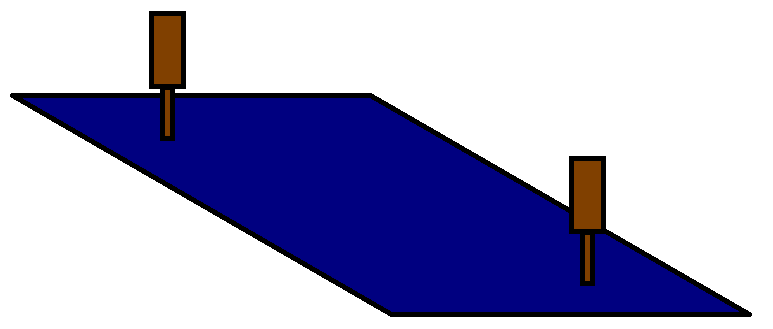
\includegraphics[width=0.60\textwidth]
	{./pictures/interference.png}

	\caption{\small{Dos fuentes puntuales sobre un fluido.}}
	
	\label{fig:doppler}
\end{figure}
%.........................................................................


Por simplicidad se describirá la oscilación producida por las fuentes como
una onda radial de la forma

%.........................................................................
%Radial wave
\eq{eq:radial_wave}
{z(r, t) = A_0\sin\pr{\omega t - k r } = A_0\sin\cor{2\pi \pr{\frac{t}{f} - \frac{r}{\lambda} }}}
%.........................................................................

donde $z(r, t)$ es la función de amplitud en $z$ de la onda, $A_0$ la 
amplitud máxima del desplazamiento, $\omega$ la frecuencia angular, $f$ la 
frecuencia y $\lambda$ la longitud de onda. El valor de $r$ es medido desde 
el origen de la perturbación, es decir, en la posición de cada fuente.
Para calcular la amplitud total se usa el principio de superposición, donde
se suman las contribuciones de cada fuente.

\

En orden para correr el código de la demostración apropiadamente, es 
necesario instalar el siguiente programa

%.........................................................................
%Installing pyaudio
\begin{listing}[style=consola, numbers=none]
\$ sudo apt-get install ffmpeg
\end{listing}
%.........................................................................

Este programa permite generar videos a partir de un conjunto de imágenes
nombradas apropiadamente.

\

A continuación de ilustra el código de la demostración


%ccccccccccccccccccccccccccccccccccccccccccccccccccccccccccccccccccccccccc
%DEMO 4_01
\begin{listing}[style=python]
# -*- coding: utf-8 -*-
#!/usr/bin/env python
#==========================================================
# DEMOSTRACION 1
# Interferencia de Ondas
#==========================================================

#**********************************************************
#	MODULOS
#**********************************************************
import numpy as np
import os
import matplotlib.pylab as plt

#Funcion de amplitud de una fuente
def Z_amplitud(x, y, x0, y0, A0, t):
    #Posicion de la fuente
    r0 = np.array([x0, y0])
    #Posicion donde se evalua el campo
    r = np.array([x, y])
    return A0*np.sin( 2*np.pi*(t/f - np.linalg.norm(r-r0)/lamb ) )

#PARAMETROS
#frecuencia		[Hz]
f = 10.
#Longitud de onda	[m]
lamb = 1.0
#Tamano de la caja	[m]
L = 10.0
#Resolucion grid caja
NS = 100

#Posicion X fuente 1	[m]
x01 = 1.0	
#Posicion Y fuente 1	[m]
y01 = 2.0
#Amplitud fuente 1	[m]
A01 = 0.1
#Posicion X fuente 2	[m]
x02 = 5.0	
#Posicion Y fuente 2	[m]
y02 = 5.0
#Amplitud fuente 2	[m]
A02 = 0.1

#Tiempo final		[s]
Tmax = 20.0
#Numero de intervalos
Nstep = 41

#GRID Y EVOLUCION
XM = np.linspace( 0, L, NS )
YM = np.linspace( 0, L, NS )

k = 0
for t in np.linspace( 0, Tmax, Nstep ):
    Z = np.zeros( (NS,NS) )
    for i in xrange( 0, NS ):
	for j in xrange( 0, NS ):
	    x = XM[i]
	    y = YM[j]
	    Z[-j,i] = Z_amplitud(x, y, x01, y01, A01, t) + \
	    Z_amplitud(x, y, x02, y02, A02, t)
	    
    plt.xlabel( 'X (0,L)' )
    plt.ylabel( 'Y (0,L)' )
    plt.title( 'Interfencia: t=%f'%(t) )
    plt.imshow( Z, extent = (0,L,0,L), vmax = A01 + A02 )
    print t
    fname='_tmp-%03d.png'%k
    k+=1
    plt.savefig(fname)
    plt.close()

print 'Making movie animation.mpg - this make take a while'
os.system("ffmpeg -f image2 -i _tmp-%03d.png  video.mpg")
os.system('rm -rf *.png')
\end{listing}
%ccccccccccccccccccccccccccccccccccccccccccccccccccccccccccccccccccccccccc

El resultado obtenido es un video donde se ilustra la evolución del patrón
de interferencia. Una toma del video es realizada en la siguiente figura


%.........................................................................
%Doppler signal
\begin{figure}[htbp]
	\centering
	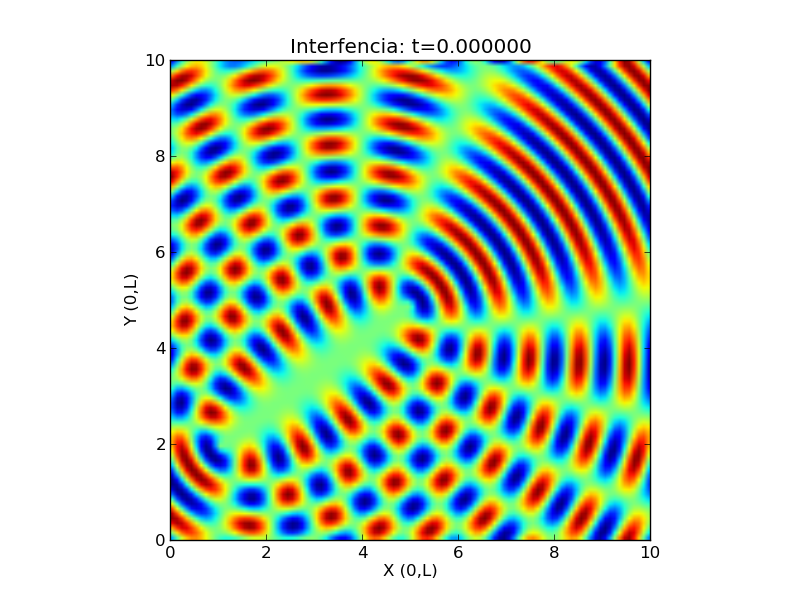
\includegraphics[width=0.90\textwidth]
	{./pictures/Two_Sources.png}

	\caption{\small{Patrón de interferencia de dos fuentes.}}
	
	\label{fig:interference}
\end{figure}
%.........................................................................


A continuación se explica cada parte del código


%ccccccccccccccccccccccccccccccccccccccccccccccccccccccccccccccccccccccccc
%DEMO 4_01
\begin{listing}[style=python, numbers = none]
import numpy as np
import os
import matplotlib.pylab as plt
\end{listing}
%ccccccccccccccccccccccccccccccccccccccccccccccccccccccccccccccccccccccccc
Se cargan las librerías estándar.


%ccccccccccccccccccccccccccccccccccccccccccccccccccccccccccccccccccccccccc
%DEMO 4_01
\begin{listing}[style=python, numbers = none]
#Funcion de amplitud de una fuente
def Z_amplitud(x, y, x0, y0, A0, t):
    #Posicion de la fuente
    r0 = np.array([x0, y0])
    #Posicion donde se evalua el campo
    r = np.array([x, y])
    return A0*np.sin( 2*np.pi*(t/f - np.linalg.norm(r-r0)/lamb ) )
\end{listing}
%ccccccccccccccccccccccccccccccccccccccccccccccccccccccccccccccccccccccccc
Se define la función de amplitud para una fuente puntual. Los argumentos
son, la coordenada del punto donde se desea evaluar el campo (\texttt{x},
\texttt{y}), la coordenada de la fuente (\texttt{x0}, \texttt{y0}), la
amplitud de la oscilación \texttt{A0} y el tiempo actual \texttt{t}.


%ccccccccccccccccccccccccccccccccccccccccccccccccccccccccccccccccccccccccc
%DEMO 4_01
\begin{listing}[style=python, numbers = none]
#PARAMETROS
#frecuencia		[Hz]
f = 10.
#Longitud de onda	[m]
lamb = 1.0
#Tamano de la caja	[m]
L = 10.0
#Resolucion grid caja
NS = 100

#Posicion X fuente 1	[m]
x01 = 1.0	
#Posicion Y fuente 1	[m]
y01 = 2.0
#Amplitud fuente 1	[m]
A01 = 0.1
#Posicion X fuente 2	[m]
x02 = 5.0	
#Posicion Y fuente 2	[m]
y02 = 5.0
#Amplitud fuente 2	[m]
A02 = 0.1

#Tiempo final		[s]
Tmax = 20.0
#Numero de intervalos
Nstep = 41

#GRID Y EVOLUCION
XM = np.linspace( 0, L, NS )
YM = np.linspace( 0, L, NS )
\end{listing}
%ccccccccccccccccccccccccccccccccccccccccccccccccccccccccccccccccccccccccc
Se definen todos los parámetros del sistema, incluyendo el grid donde se 
evaluará el campo de desplazamiento de la onda.


%ccccccccccccccccccccccccccccccccccccccccccccccccccccccccccccccccccccccccc
%DEMO 4_01
\begin{listing}[style=python, numbers = none]
k = 0
for t in np.linspace( 0, Tmax, Nstep ):
    Z = np.zeros( (NS,NS) )
    for i in xrange( 0, NS ):
	for j in xrange( 0, NS ):
	    x = XM[i]
	    y = YM[j]
	    Z[-j,i] = Z_amplitud(x, y, x01, y01, A01, t) + \
	    Z_amplitud(x, y, x02, y02, A02, t)

    plt.xlabel( 'X (0,L)' )
    plt.ylabel( 'Y (0,L)' )
    plt.title( 'Interfencia: t=%f'%(t) )
    plt.imshow( Z, extent = (0,L,0,L), vmax = A01 + A02 )
    print t
    fname='_tmp-%03d.png'%k
    k+=1
    plt.savefig(fname)
    plt.close()
\end{listing}
%ccccccccccccccccccccccccccccccccccccccccccccccccccccccccccccccccccccccccc
Se realiza un ciclo \texttt{for} para la iteración de cada tiempo del 
sistema. Se hace un barrido sobre las dos coordenadas \texttt{x = XM[i]},
\texttt{y = YM[j]} y se calcula el valor del campo de las dos fuentes 
\texttt{Z[-j,i] = Z\_amplitud(x, y, x01, y01, A01, t) + 
Z\_amplitud(x, y, x02, y02, A02, t)}. Usando la función 
\texttt{plt.savefig(fname)} de \matplotlib, se guarda la grafica del campo
en el tiempo actual, con el nombre \texttt{'\_tmp-\%03d.png'\%k} donde 
\texttt{k} es un contador entero. Una vez guardada la gráfica, se cierra
el entorno gráfico actual con la función \texttt{plt.close()} y se procede
a calcular el siguiente tiempo.



%ccccccccccccccccccccccccccccccccccccccccccccccccccccccccccccccccccccccccc
%DEMO 4_01
\begin{listing}[style=python, numbers = none]
os.system("ffmpeg -f image2 -i _tmp-%03d.png  video.mpg")
os.system('rm -rf *.png')
\end{listing}
%ccccccccccccccccccccccccccccccccccccccccccccccccccccccccccccccccccccccccc
Finalmente se realiza el video a partir del programa \texttt{ffmpeg}. El 
formato de uso puede ser consultado en la página oficial del proyecto 
\footnote{\url{http://www.ffmpeg.org/}}, aunque los parámetros usados en
este código son óptimos para la generación de videos en \python.

%*************************************************************************



\newpage
%*************************************************************************
\section{Ejercicios}
\label{sec:ejercicios}

%.........................................................................
\subsection*{Ejercicio 1 \large{$\pr{\star}$}}

\textbf{Interferencia de 3 fuentes con reflexión}

Considere el mismo sistema de la demostración 1, pero con tres fuentes 
puntuales. 
%Mass-Spring system
\begin{figure}[htbp]
	\centering
	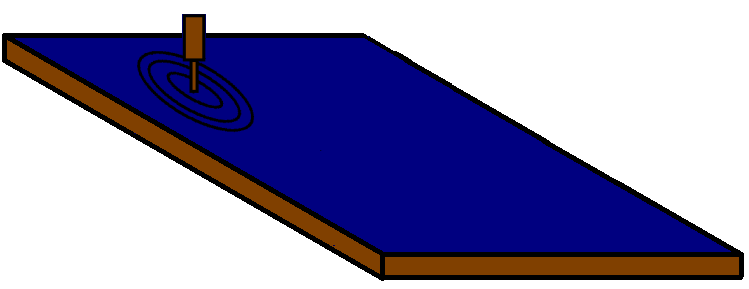
\includegraphics[width=0.60\textwidth]
	{./pictures/interference_reflex.png}

	\caption{\small{Sistema masa resorte.}}
	
	\label{fig:mass_spring}
\end{figure}

A partir de este sistema, hacer un código que realice un video donde se
muestre el patrón de interferencia en el tiempo de las tres fuentes, además
se debe considerar reflexión en las paredes de la caja. 

\textit{Hint:} para simular la reflexión de las ondas, puede considerar 
fuentes ficticias en el exterior de la caja que tengan posiciones simétricas
respecto a las fuentes originales.
%.........................................................................


%.........................................................................
\subsection*{Ejercicio 2 \large{$\pr{\star}$}}

\textbf{Interferencia de fuentes sonnoras}

Considere un sistema análogo a la demostración 1, donde el medio es aire y
las perturbaciones son sonoras. En este caso las ondas son longitudinales,
pero sigue siendo válido el principio de superposición.

\

Usando la librería \texttt{AudioLib} \footnote{ver ejemplo de uso en 
demostración 2 del capítulo 3 (Efecto Dopler)} simule el audio que sería 
percibido por una persona que camina en una habitación cuadrada de lado $L$
cuando las dos fuentes están prendidas. 

\begin{itemize}
\item Genere un audio .wav para dos frecuencias armónicas, es decir, que 
satisfacen una relación entera.
\item Genere un audio .wav para dos frecuencias no armónicas.
\end{itemize}

La función de desplazamiento del observador es de libre elección, puede 
ser un movimiento unidimensional acelerado o a velocidad constante, puede
ser en dos dimensiones. La única condición es que debe ser a una velocidad 
promedio para una persona (no comparable a la velocidad del sonido!). 
Recuerda que se quiere simular una situación físicamente plausible.

\

\textit{Hint:} todos los valores de los parámetros son de libre elección,
la única condición es coherencia física en el resultado. La función 
\texttt{savewav} de \texttt{AudioLib} puede ser de utilidad (en ipython,
después de importar la librería y crear un objeto \texttt{audio}, 
escribir \texttt{<object\_name>.savewav?}).
%.........................................................................


%.........................................................................
\subsection*{Ejercicio 3 \large{$\pr{\star}$}}

\textbf{Simulación de difracción}

%Mass-Spring system
\begin{figure}[htbp]
	\centering
	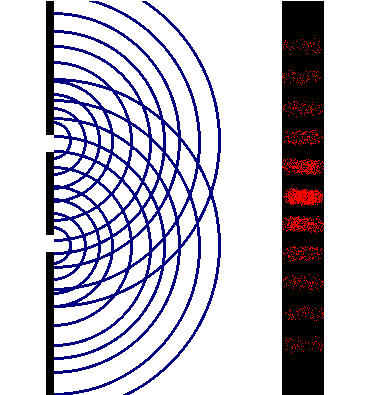
\includegraphics[width=0.50\textwidth]
	{./pictures/diffraction.png}

	\caption{\small{Sistema masa resorte.}}
	
	\label{fig:mass_spring}
\end{figure}
%.........................................................................

%*************************************************************************